%!TEX root = main.tex
\section{Results}
\subsection{With and without Olympic Games}
Choosing $\beta=2$, $\gamma=0.5$ and an average transfer probability of $0.005$ we can run a simulation with and without the Olympic Games occurring with the previously described characteristics. We assume that the infection breaks out on the first day of the games in Rio De Janeiro. We set the initial infected population to 1000. In the following we will look at the SIR curves of 6 major cities.

With the Olympics occurring we get the following curves:
\begin{figure}[H]
	\centering
	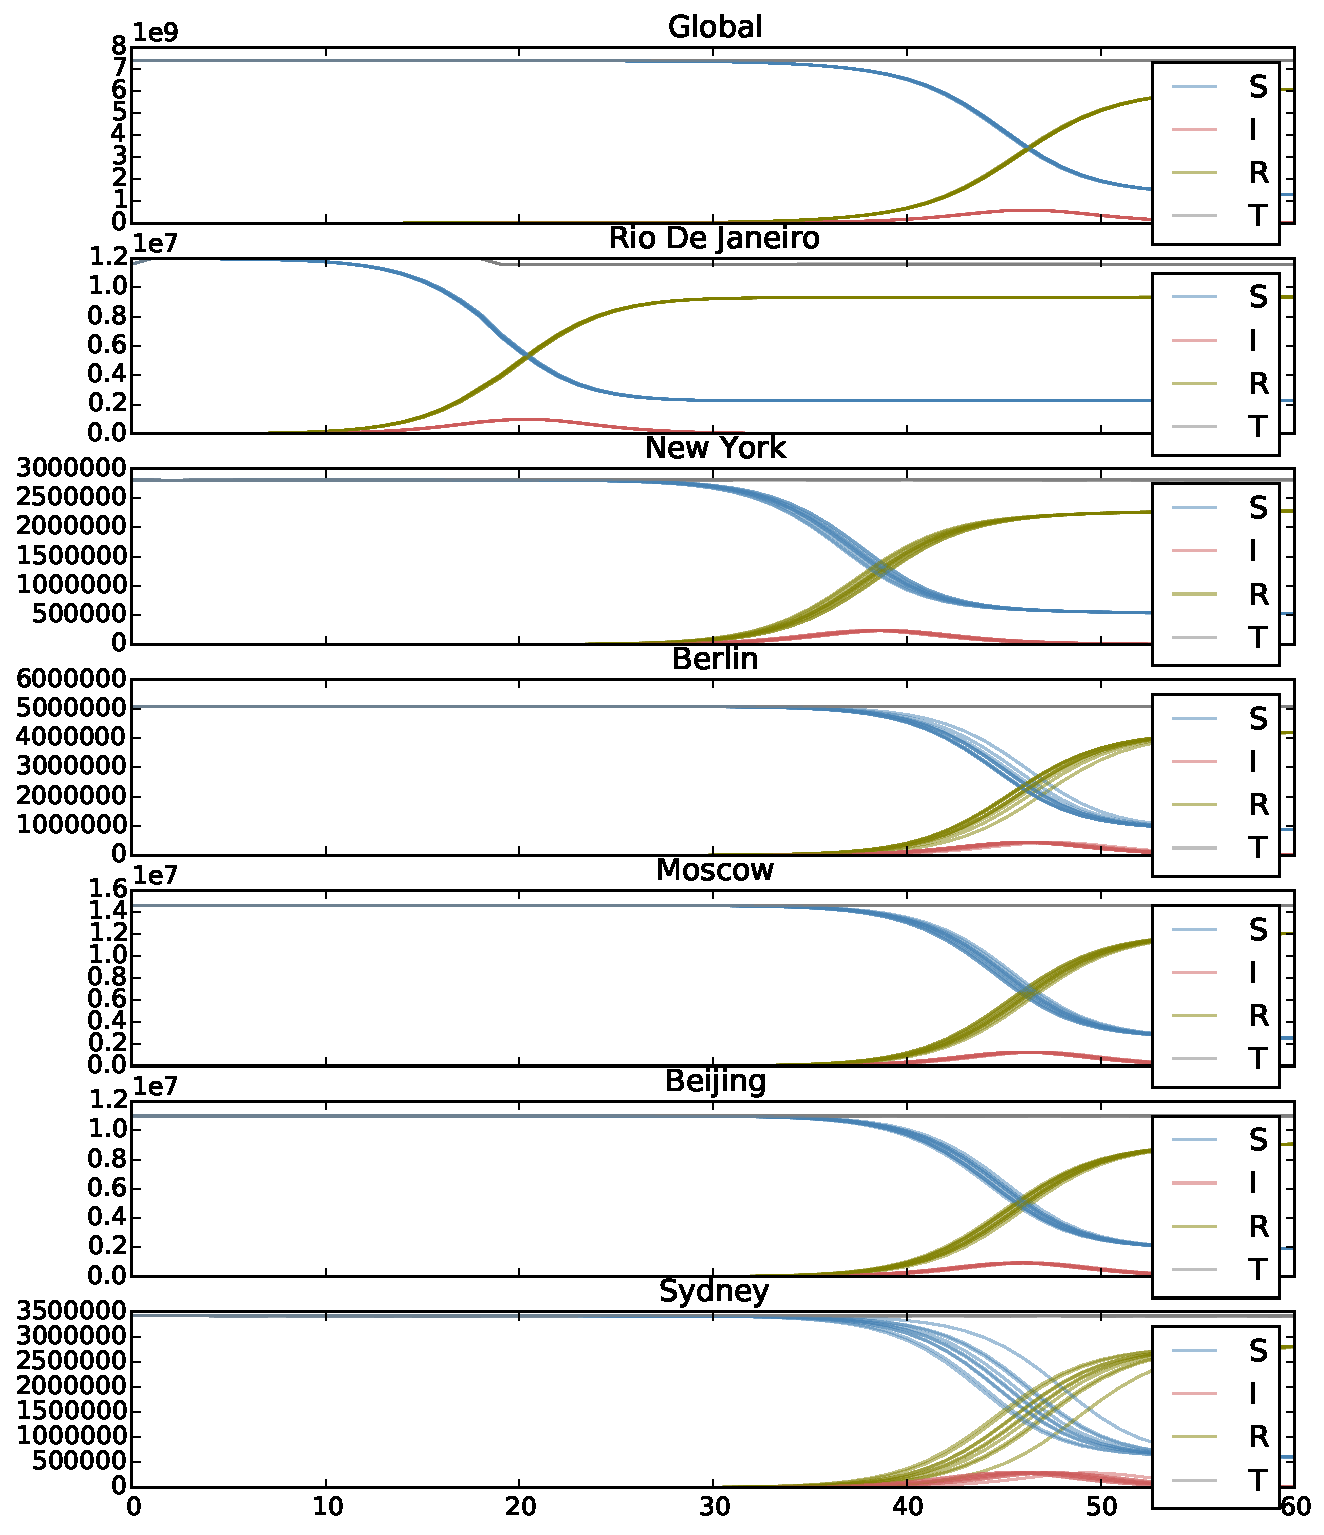
\includegraphics[width=1.0 \linewidth]{plots/rio-0-18-380000.pdf}
	\caption{10 simulations with Olympic Games. Time in days on the x-axis and number of people on the y-axis. Shown is susceptible (S), infected (I), removed (R) and total population (T).}
	\label{fig:rio-0-18-380000}
\end{figure}

From figure \ref{fig:rio-0-18-380000} it's seen that except for Rio where the infection started and New York which seems to be infected earliest, the other major cities all seem to reach peak infection rates at approximately the same time. 

\begin{figure}[H]
	\centering
	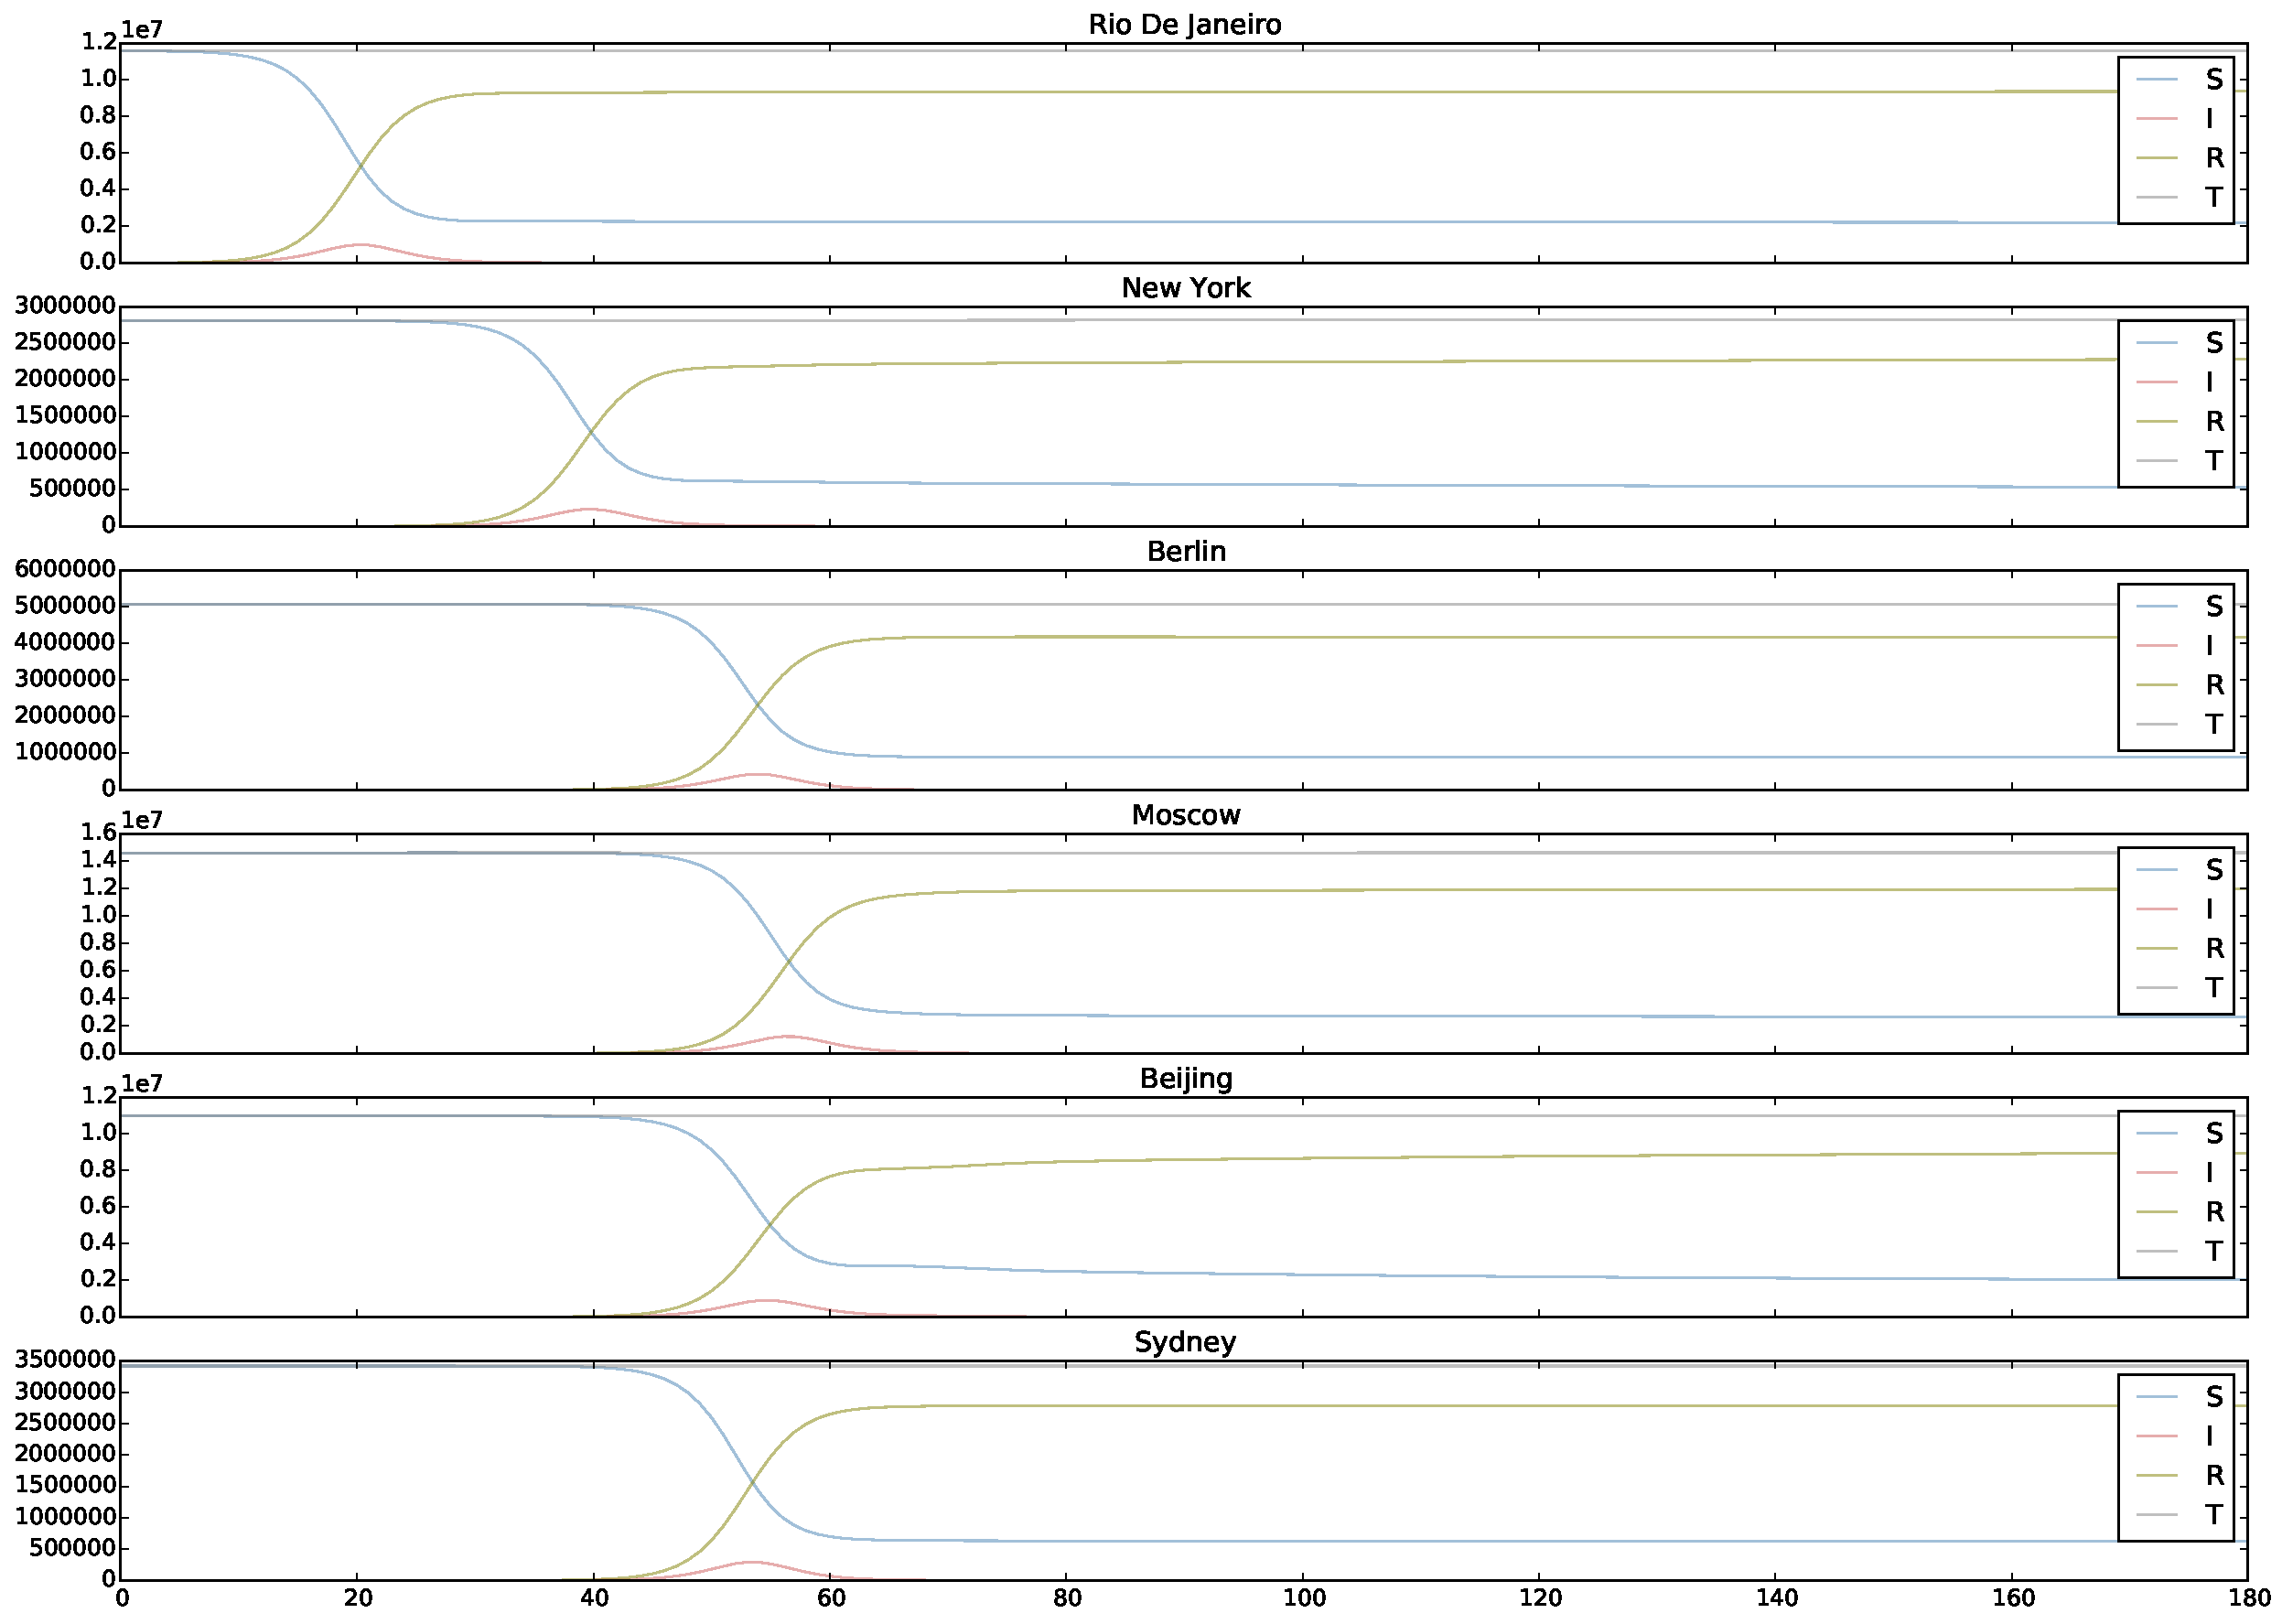
\includegraphics[width=1.0 \linewidth]{plots/no_rio.pdf}
	\caption{10 simulations without Olympic Games. Time in days on the x-axis and number of people on the y-axis}
	\label{fig:no_rio}
\end{figure}

When there is no Olympic Games, as seen in figure \ref{fig:no_rio}, the peak infections occur later, especially for Moscow, Beijing and Sydney. The is emphasized in the summary table \ref{table:olympic-summary}.

\begin{table}[H]
	\centering
	\begin{tabular}[H]{c | c | c}
Observation & With OL & Without OL \\ \hline 
 Peak amount Global [million]& $590.5\pm 0.94 (0.02)$ & $291.5 \pm 1.41 (0.01)$\\ 
 Peak time Global & $46.0\pm 0.00( 0.00)$ & $67.0 \pm 0.00 (0.00)$\\ 
 Peak time Rio & $20.2\pm 0.30( 0.26)$ & $20.0 \pm 0.00 (0.00)$\\ 
 Peak time New York & $38.6\pm 0.50( 0.52)$ & $38.3 \pm 0.59 (0.50)$\\ 
 Peak time Berlin & $46.4\pm 0.77( 0.56)$ & $53.7 \pm 0.35 (0.30)$\\ 
 Peak time Moscow & $46.1\pm 0.23( 0.23)$ & $56.3 \pm 0.35 (0.28)$\\ 
 Peak time Beijing & $46.0\pm 0.00( 0.00)$ & $55.0 \pm 0.34 (0.30)$\\ 
 Peak time Sydney & $46.3\pm 0.83( 0.73)$ & $53.3 \pm 0.48 (0.51)$
\end{tabular}
	\caption{Results of 10 simulations with and without Olympic Games. Table contains the peak times and amounts for the number of infected individuals. The standard $95\%$-confidence interval is marked with $\pm$ and the confidence interval using control variates is shown in the parenthesis.}
	\label{table:olympic-summary}
\end{table}

As mentioned one see in table \ref{table:olympic-summary} that the peak time is much less spread and generally happens earlier, when the Olympic Games happens. This is particularly apparent when comparing with the global peak time, which in the case without Olympic Games, happens statistically significantly later when comparing to the cities. While in the Olympic Games case, it is within statistical significantly, except for the Network and Rio case.

Rio doesn't have a significantly difference in peak time, this makes sense as this is where the infection starts. Adding 380000 people (out of 12 million people) doesn't make much of a difference. The New York case is also interesting

\subsection{Visualization of result}
When studying a virus outbreak it is interesting to see exactly how the virus spreads. We have thus created an animation on a world map showing where each region is represented as a dot (scaled according to the population size) and the color of the dot represents the fraction infected. With this visualization the difference between including the Olympic Games and including becomes more apparent.

\begin{figure}[H]
	\centering
	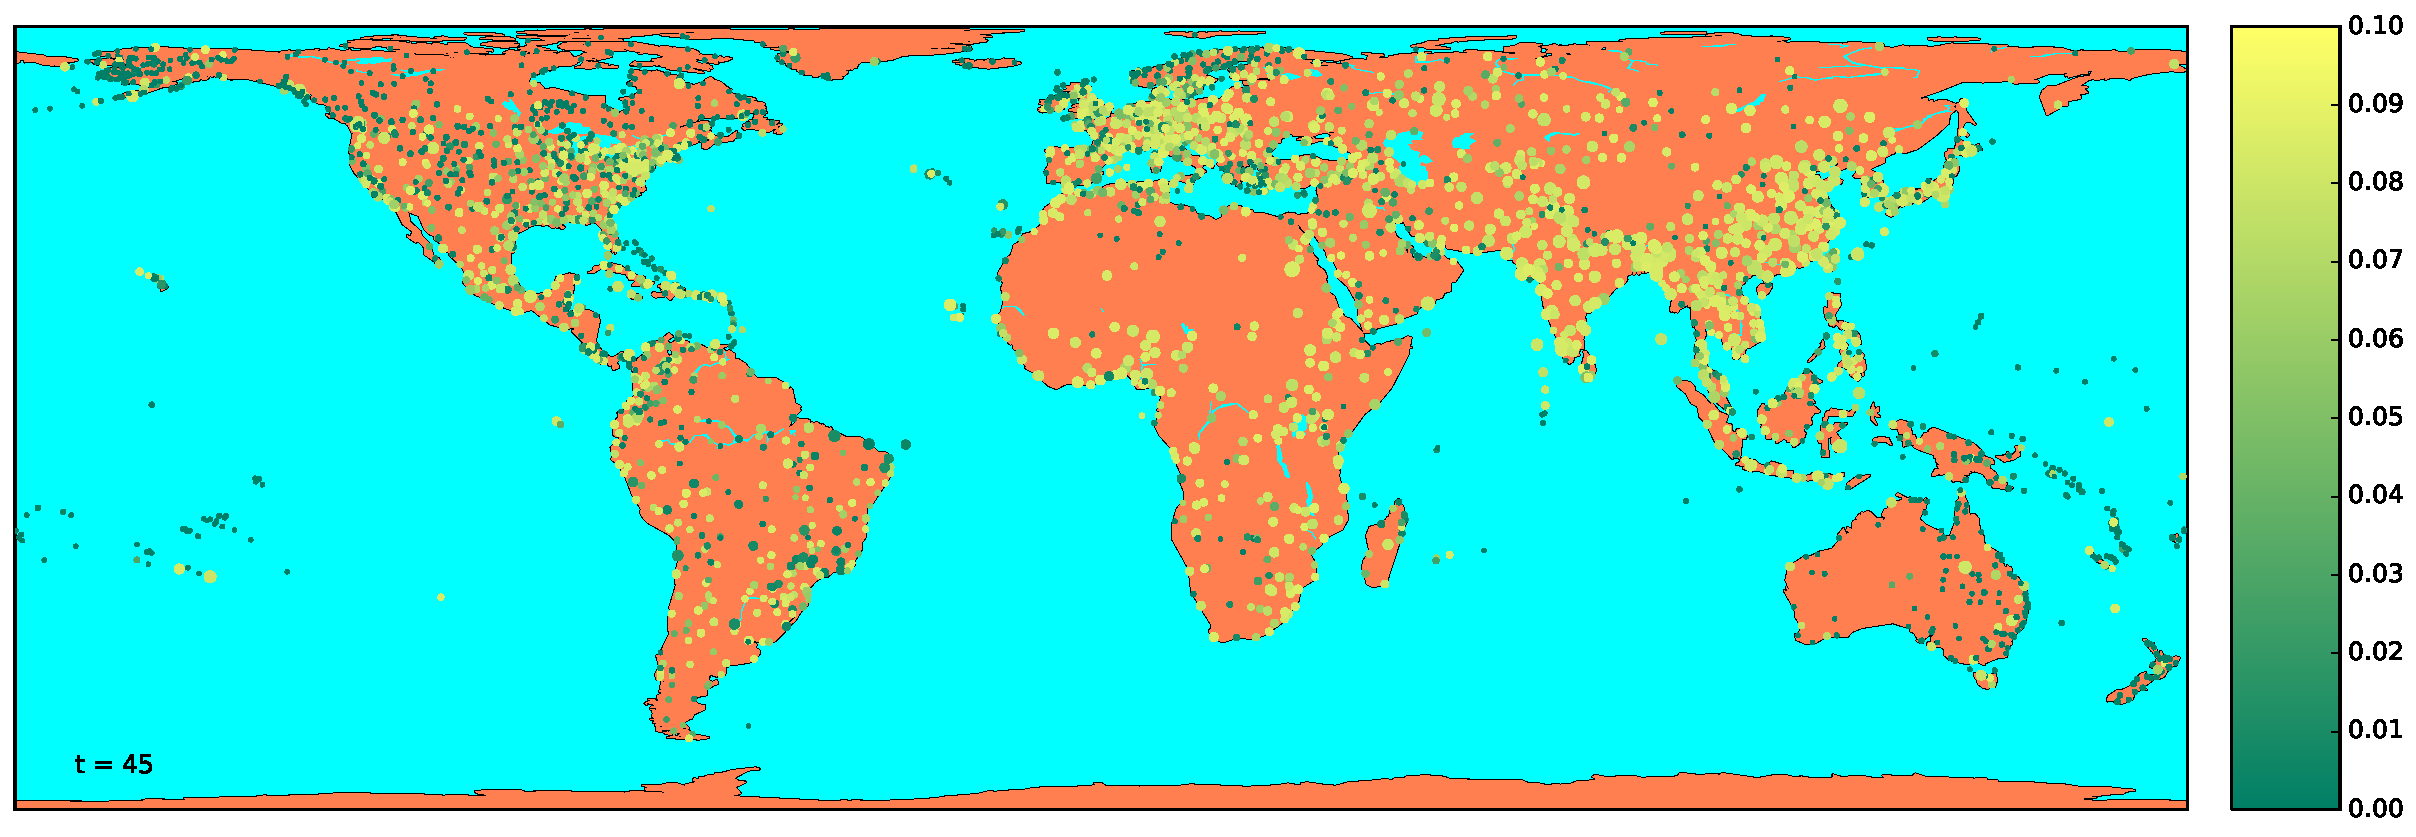
\includegraphics[width=1.0 \linewidth]{plots/gifs/frames/rio-45}
	\caption{Frame 45 of animation with Olympic Games. The full animation can be viewed as a gif at
		\url{https://andreasmadsen.github.io/course-02443-stochastic-virus-outbreaks/}}
\end{figure}

\begin{figure}[H]
	\centering
	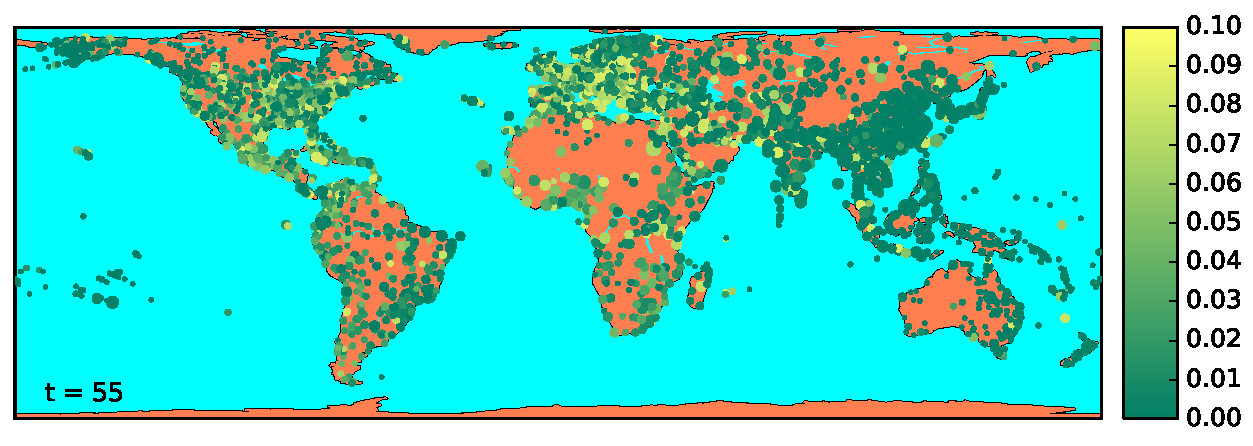
\includegraphics[width=1.0 \linewidth]{plots/gifs/frames/noRio-55}
	\caption{Frame 55 of animation without Olympic Games. The full animation can be viewed as a gif at
		\url{https://andreasmadsen.github.io/course-02443-stochastic-virus-outbreaks/}}
\end{figure}


